Este capítulo é dedicado à introdução do leitor ao principal tópico de estudo do projeto e assim mostrar
algumas aplicações onde este é usado, além de apresentar os desafios relacionados à estas aplicações.

\section{Resposta ao Impulso de Ambiente Acústico e suas Aplicações}

Dentre os diversos tópicos na grande área de estudo de sinais de áudio, destaca-se a detecção e reconhecimento de fontes acústicas no espaço físico.
Um caso específico deste tópico é sobre sinais de voz gravados em ambientes fechados, onde um ou mais microfones são posicionados na sala afastados
da fonte sonora, normalmente uma pessoa que performa a gravação.
Estes sinais são corrompidos pela reverberação do ambiente, que surge a partir da sobreposição da onda sonora anecoica que chega ao microfone com a 
onda sonora atenuada e refletida nas paredes do ambiente fechado. 

\begin{figure} [H]
    \begin{subfigure}{.5\textwidth}
        \centering
        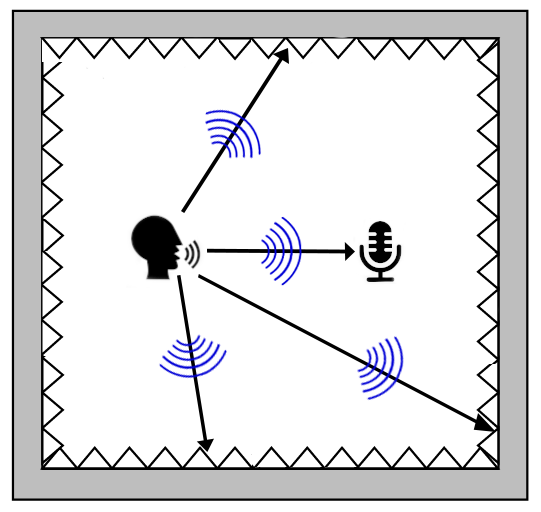
\includegraphics[scale=0.4]{camara_anecoica.png}
        \caption{Sala anecoica}    
    \end{subfigure}
    \begin{subfigure}{.5\textwidth}
        \centering
        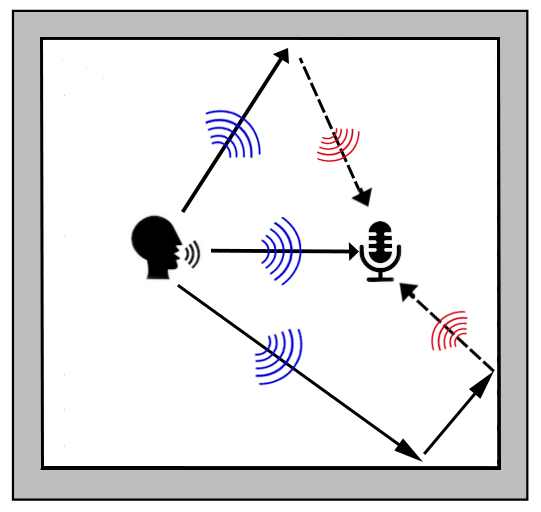
\includegraphics[scale=0.4]{camara_reverb.png}    
        \caption{Sala reverberante}    
    \end{subfigure}
    \caption{Representação de uma sala anecoica e reverberante}
    \label{fig:Rooms}
\end{figure}

Observa-se na figura \ref{fig:Rooms} uma representação de uma sala anecoica, onde o único áudio capturado pelo microfone é a onda sonora direta
enviada pela fonte, sem nenhuma reflexão do ambiente; já na sala reverberante, nota-se que o áudio capturado será uma combinação da onda sonora direta
com as refletidas nas paredes. 
Este sinal reverberado pode ser modelado da seguinte forma:

\begin{equation}
    Y(t) = s(t) \ast h(t) + n(t)
\end{equation}

% ### TODO: [FIGURA] exemplificando voz reverberada e figura mostrando o que é RIR

Onde $Y(t)$ representa o sinal de voz em campo distante, $s(t)$ o sinal de voz anecoico, $h(t)$ a RIR e $n(t)$ o sinal de ruído que pode
estar presente no ambiente.
Dessa forma, é possível inferir que a RIR representa o modelo acústico de uma sala, para uma determinada combinação de fatores do ambiente, incluindo: 
temperatura e umidade relativa do ar, pressão atmosférica, material das paredes e posicionamento de móveis.
Reverberação causa degradação do sinal de voz, levando à perda de clareza na comunicação \cite{Speech_intellig_hear} e à redução da performance
de sistemas de reconhecimento de voz \cite{reverb_sup_speech_reg}. Este problema demonstra a necessidade de identificar dinamicamente o modelo acústico
do ambiente para que possam ser mitigadas as perdas nas amostras de voz gravadas e assim facilitar os algoritmos que usam esses sinais.

% ### TODO: completar isso, exemplificar reconhecimento de voz e separação de fontes
Este projeto é focado no estudo de uma forma de gerar RIRs simuladas a partir de RIRs reais devido à sua importância para diversas
aplicações usadas atualmente na indústria. Uma de suas aplicações é na análise e desenvolvimento de algoritmos de 
reconhecimento de voz robusta \cite{reverb_sup_speech_reg}, onde é necessário inferir a RIR para que possa ser feita a comparação entre
a supressão da reverberação ideal com a cega.
Outra aplicação da RIR é para desenvolvimento de algoritmos para localização e separação de fontes sonoras \cite{Source_sep_RIR},
onde as RIRs são usadas no auxílio do mapeamento acústico de ambientes reverberante através de algoritmos de separação de fonte às cegas.

\section{Desafios correlacionados a RIR}

% ### TODO: aplicações em deep learning e pq falta dado
